% !TeX root = ../main.tex
% -*- coding: utf-8 -*-
% !TeX root = ../main.tex
% -*- coding: utf-8 -*-

\chapter{绪论}
\label{chpt:introduction}
本章首先阐述本文的选题背景和意义,然后阐述论文的主要工作和创新点,最后介绍论文结构安排。

\section{研究背景与意义}
在软件生命周期中,随着外部环境的改变和用户需求的不断更新,软件开发人员必须不断修改软件系统以适应新的
需求。这种改变包括对软件错误的修复、新功能的添加和新的软件开发技术的应用等。然而,随着软件系统的不断
改变,代码结构变得越来越复杂,导致软件质量的逐渐下降。在软件演化过程中,为了保证软件质量,提高用户体
验,开发者有必要对软件系统进行维护。

软件维护是指在软件发布后,为了修复错误、改善设计、提升性能等提高软件质量的目的而进行的软件修改
~\cite{IEEE1219}。在现代软件系统中,软件维护是贯穿软件生命周期的软件活动,具有周期长、人员流动性强的
特点。软件维护人员需要花费大量的时间来理解和维护软件~\cite{Bansiya2002}。研究者发现,在整个软件生命周期
中,软件维护和演化的成本占总成本的80\%以上~\cite{guimaraes1983managing, coleman1994using}。由于软件
维护占据整个生命周期的大部分,因此不能快速和可靠地维护软件往往带来巨大的损失。

\subsection{软件维护的类型}

\begin{figure}
  \centering
  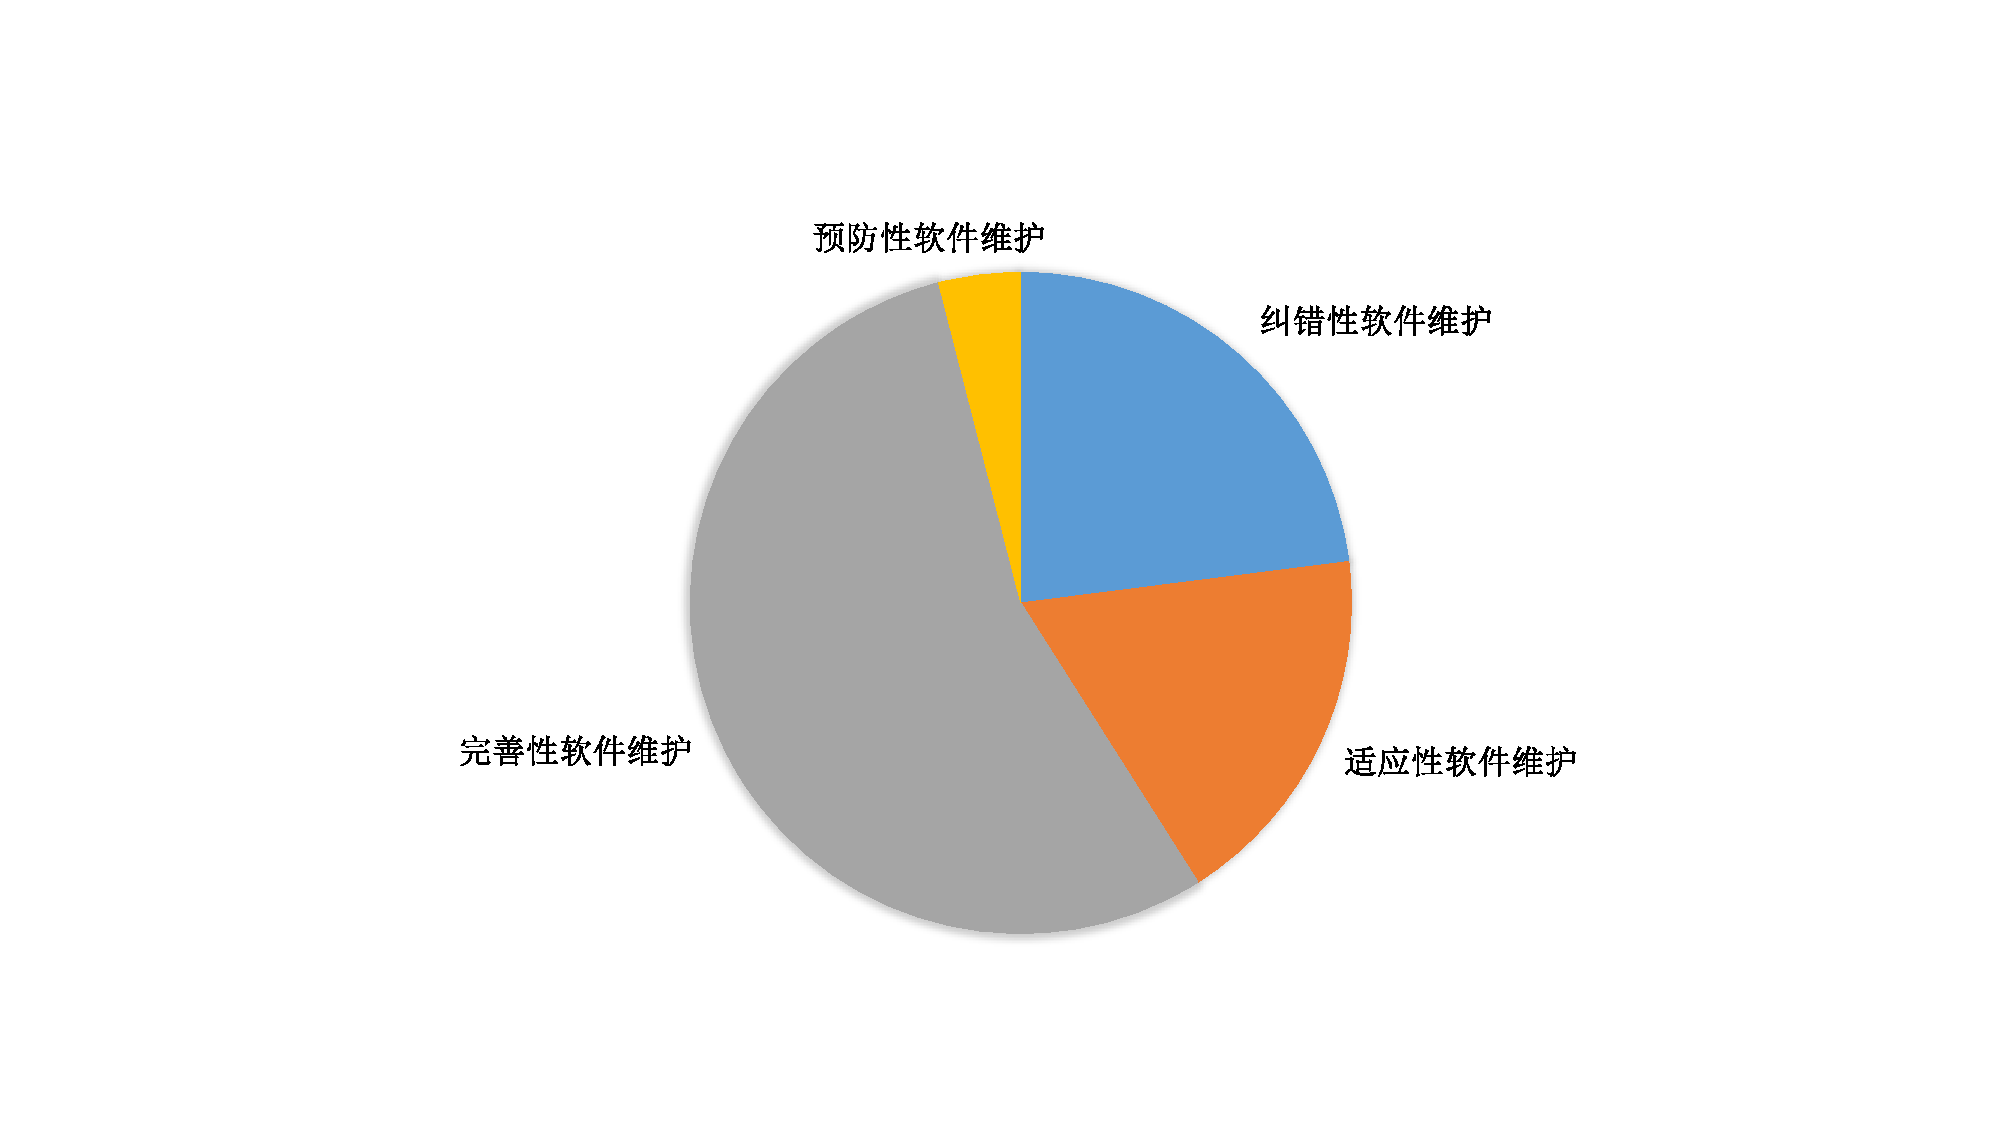
\includegraphics[width=0.6\linewidth]{maintenance.pdf}  
  \caption{\label{fig:maintenance}软件维护类型}
\end{figure}

如图~\ref{fig:maintenance}所示,软件维护可分为四种类型:纠错性软件维护、适应性软件维护、完善性软件维
护和预防性软件维护~\cite{lientz1978characteristics}。

\begin{itemize}
  \item 纠错性软件维护是提高软件可靠性的重要手段,指的是纠正在软件开发过程中未被发现的,实际应用中出
现软件行为与预期不相同的错误。由于软件开发过程中很难做到发现所有潜在的错误,因此在软件系统的实际应用
中,可能会触发软件错误,导致系统不能正常运行,可能给经济和社会带来巨大的损失。根据美国的标准与技术研
究报告,软件缺陷为美国带来每年高达600亿美元的损失,而即使发现软件缺陷则会为美国每年节约超220亿美元
~\cite{strate2013literature}。纠错性软件维护通常是在软件发生缺陷时进行的对软件缺陷的定位、诊断和修
复。
  \item 完善性软件维护则是关系到软件系统质量的重要方面,包括改进程序设计、提升软件运行的效率和性能
等。在软件的使用过程中,随着外部环境的不断变化和用户需求的不断提升,用户对系统的功能和性能要求也逐步
提高。然而,由于缺陷修复和新功能的添加,程序变得越来越复杂,导致软件质量逐渐降低。完善性软件维护通过
改进软件设计、提高运行效率等手段来提高软质量,在延长软件寿命的同时降低软件维护成本。
  \item 适应性维护通常是为了让软件适应技术和外部环境的变化而进行的。一方面,随着软件开发技术的发展和
操作系统版本的更迭,软件维护人员需要不断改进软件从而适应新的技术环境;另一方面,硬件环境的更新带来系
统性能和效率的大幅度提升,这就要求软件维护人员有计划性地修改软件系统,从而适应新的硬件环境。
  \item 预防性软件维护是为了适应未来软件的环境变化,将被动转化为主动而添加的新功能。对软件系统的维护
工作并不一定只能在软件系统出了错误或是用户提出需求才能执行,合理的预防性的软件维护可以将软件维护的成
本降低,提高用户的使用体验。对正在使用中的软件系统,预防性软件维护考虑到将来可能发生的修改,对软件系
统实施有计划性的修改,从而使其容易适应环境和需求的改变,不易被淘汰。
\end{itemize}

由图~\ref{fig:maintenance}中可以看出,纠错性和完善性软件维护是最主要的两种软件维护手段,占软件维护总
量约75\%。纠错性软件维护是保证软件正确性的重要手段,是完善性软件维护的基础;同时,完善性软件维护通过
改进软件设计、提高软件质量的方式,让代码更易读,提高缺陷定位和错误修复的效率。


\subsection{基于数据驱动的软件维护}
由于当代软件系统具备代码规模大、迭代周期短等特点,人工软件维护变得越来越困难。一方面,软件维护依赖于程序
员对软件系统细致的理解。然而,随着软件系统规模的扩大,代码的复杂度也越来越高,即便是经验丰富的软件维
护人员也很难完全掌握整个软件系统,导致人工进行软件维护变得越来越困难,且其效果也容易受到个体思维的影
响。另一方面,软件维护通常具备周期长、人员流动性大、工作枯燥繁复等特点,人工进行软件维护
不但需要大量的人力资源,其效率也会随着软件复杂性的提升而不断降低,导致软件维护的时间和人力成本较高,
很难满足当代软件系统快速迭代的要求。

自动化的软件维护可以解决人工维护的效率低、易受个体思维影响的缺点,因此,很多研究者致力于提出各种自动
化、半自动化技术来提高软件维护的效率和性能。例如,在纠错性软件维护方面,研究者们提出用自动化测试技术
来代替传统的人工测试,从而解决人工测试中的遗漏、思维惯性等问题,使测试更快、更可靠、更便宜。在完善性
软件维护方面,大多数集成开发环境,如Eclipse和IntelliJ IDEA等,提供了软件重构的支持工具作为插件。 当
开发人员需要重构时,首先选择待重构代码,然后选定软件重构类型以及必要的输入(如函数重命名操作中的新函
数名),重构工具可以替代软件维护人员完成剩下的工作。这样的工具为自动和半自动化软件重构提供了基础,是
软件重构被广泛应用的重要因素~\cite{griswold1993automated,tip2003refactoring,mens2005formalizing}。

然而,由于软件维护的复杂性,研究者很难制定一套完整而严密的规则来解决软件维护中的难题,因此当前的软件
维护工作很难被完全自动化的技术所完成。例如,虽然自动化测试技术可以大量的减少枯燥重复的工作,提高软件
测试的效率,然而对测试结果的判定依赖软件维护人员,自动化判断测试用例的预期表现仍然是尚待解决的难题。
同样,基于集成环境的软件重构工具通过开发工具来为特定类型的手动重构操作提供技术支持
~\cite{fowler1999refactoring, murphy2012we}。虽然很多编辑器和集成开发环境集成了这类重构支持工具,其
作用仅仅是替软件维护人员执行指定的重构操作,仍然依赖于软件维护人员来识别软件重构机会和选择软件重构操
作。因此,手动重构的过程较为复杂和乏味,软件维护人员需要花费大量的时间和精力指定需要被执行的软件重构
操作。

数据挖掘对于这种存在内部规律但却很难通过人为制定完整规则来解决的难题提供了一种新的解决思路,即挖掘数
据中潜在的规律作为解决方案。成熟的开源社区和版本控制工具(如CVS、Git、SVN等)为研究者们提供了大量的
可研究数据,包括软件系统的版本、规模、复杂度、修改等。从数据的角度来理解软件系统,将软件维护问题转换
为数据挖掘问题,既避免了对软件维护人员经验的依赖性,又提高了维护效率,减少了时间和人力的成本,因此成
为了近几年软件工程的研究热点。随着信息化的发展,大量的软件代码可以被研究使用,与软件相关数据的价值逐
渐被研究者认可。机器学习和数据挖掘算法被广泛应用于缺陷预测
~\cite{menzies2007data,drown2009evolutionary,khoshgoftaar2010attribute}、缺陷定位
~\cite{malcov2013,nnfault2013}、补丁生成~\cite{martinez2015mining, long2016automatic}等方面。本文主
要针对纠错性软件维护和完善性软件维护中的关键技术,使用数据挖掘提供解决方案,为软件维护人员减少时间和
人力的成本,从而适应当代软件系统提高可靠性和实现快速迭代的需求。

\iffalse
在程序修复方面,Martinez等人~\cite{martinez2015mining}通过挖掘软件仓库中的修复数据,为抽象语法树的修
改和错误修复之间的关系建模,预测修复错误的概率。Long~\cite{long2016automatic}等提出通过挖掘成功修复
错误的补丁,为每个成功的补丁提取了面向修改和数值的特征,前者表示程序修改和周围代码的关系,后者表示修
改前后变量数值的改变;最后通过最大似然来预测补丁可能能够成功修复错误的概率。
\fi

\section{研究内容与创新点}
本文研究内容主要针对软件维护中两种主要的软件维护类型,即纠错性和完善性软件维护。纠错性软件维护是保证软
件正确性的重要手段,然而在纠错性维护后,虽然软件系统的正确性得以保障,但对软件系统的修改可能会导致软
件系统设计的偏离,使得软件质量降低。为了提高软件质量,通常需要后续进行完善性软件维护。

首先,为了保证软件系统的正确性,以测试用例执行作为数据基础,提出了基于Relief特征选择和分支覆盖特征谱
的缺陷定位技术。然后,为了完善软件系统设计,以开源软件仓库中的重构实例作为数据基础,针对软件系统维护
中最常见的两种软件重构操作--函数抽取和重命名重构,提出了基于数据挖掘的重构机会推荐方法。本文研宄内容
如下:

(1)基于特征选择的缺陷定位

为了提高纠错性软件维护的效率,本文研究了基于覆盖分析的缺陷定位方法(CBFL),其核心思想是被失效用
例执行越多、成功用例执行越少的代码可疑度越高~\cite{jones2005empirical}。其方法通常是收集测试用例在执
行过程中的语句、谓词或分支等覆盖信息并统计执行结果,然后根据特定的可疑度计算公式来计算代码的可疑度。
该方法用较低的计算成本计算代码的可疑度,并按照可疑度大小由高至低推荐给软件维护人员。然而,软件系统中
可能存在不止一个错误,导致测试用例失效原因也可能不止一个。基于覆盖率的缺陷定位方法,忽略了不同软件错
误之间的相互影响,因此可能导致准确性降低。

Kira等人~\cite{kira1992feature}最早提出利用相关统计量度量特征的重要性,该方法为每个测试用例分别寻找
距离最近的同类和异类,距离同类越近、距离异类越远的特征被认为越能够区分不同类别的样本,因此对样本的类
别越重要。本文引入相关统计量的概念,通过将测试用例执行的覆盖信息作为特征,测试用例执行结果作为标签,
将原问题转化为数据挖掘问题,从而推测特征(代码)对执行结果的重要性。基于由相同软件错误引发的失效用例
其覆盖信息可能相似的思想,本文通过为每个测试用例选择距离最近的同类/异类样本,在很大程度上避免了由不
同错误引发的失效样例,从而提高可疑度计算的准确性。

(2)基于梯度提升决策树的函数抽取重构机会推荐

为了提高完善性软件维护的效率,本文面向最常见的软件重构操作--函数抽取重构操作,提出基于梯度上升决策树
的重构机会推荐。当前基于软件度量和代码切片的重构机会推荐方法往往依据特定的软件度量进行排序推荐,违背
了软件重构原因的多样性和复杂性~\cite{silva2016we}。为了探究函数抽取重构的根本原因,本文通过观察开源
软件重构实例,将函数抽取重构作为训练数据,从模型的角度探讨函数抽取重构的原因,并为软件维护人员推荐重
构操作。

在训练阶段,本文收集大量的开源函数抽取重构实例作为正样本,并随机生成等比例的负样本作为训练数据。本文
提出基于软件质量概念的特征提取算法,融合了内聚度、耦合度、复杂度三个重要概念,并考虑了多种程序元素,
如变量、类型、函数调用、包等,使用梯度提升决策树和逻辑斯特回归的融合模型进行训练。在预测阶段,首先为
给定函数体生成所有合法的候选函数抽取重构操作,然后使用该融合模型进行训练,得到每个候选操作被分为正类
的概率,并根据概率由高至低进行排序,推荐给软件维护人员。

(3)基于层次注意力的函数名推荐

在完善性软件维护阶段,为了提高软件系统的易读性和可维护性,本文面向函数重命名软件重构类型提出了基于注
意力机制的推荐模型。由于软件维护的周期长、人员流动性大的特点,易读性高的软件系统其维护成本较低。好的
函数名通常具备功能描述性强的特点,因此可以提高软件维护人员错误修复、功能添加的效率。研究表明,函数抽
取和函数重命名是最常用的两种软件重构操作。为了研究好的函数名和函数体之间的关系,本文提出使用层次注意
力网络模型为给定代码片段预测其函数名。

本文的训练数据来自于GitHub上广受欢迎的开源软件,因其在多数情况下被认为具有较强的代码规范性。每个函数
的``函数名-函数体''对被视为一个训练样本。将分词后的函数体表示为一个词序列,将每个基本块视为一个功能
子单元,根据``多个基本块子功能组成一个函数,多个词组成一个基本块''的层次结构,提出使用层次注意力
模型来拟合函数体与函数名之间的关系。在预测阶段,本文首先将给定函数体表示为上述层次结构,然后使用层次
注意力网络进行预测,最后使用集束搜索生成具有概率的函数名,并按照概率的由高至低推荐用户。

\section{论文结构安排}
\begin{figure}[htp]
  \centering
  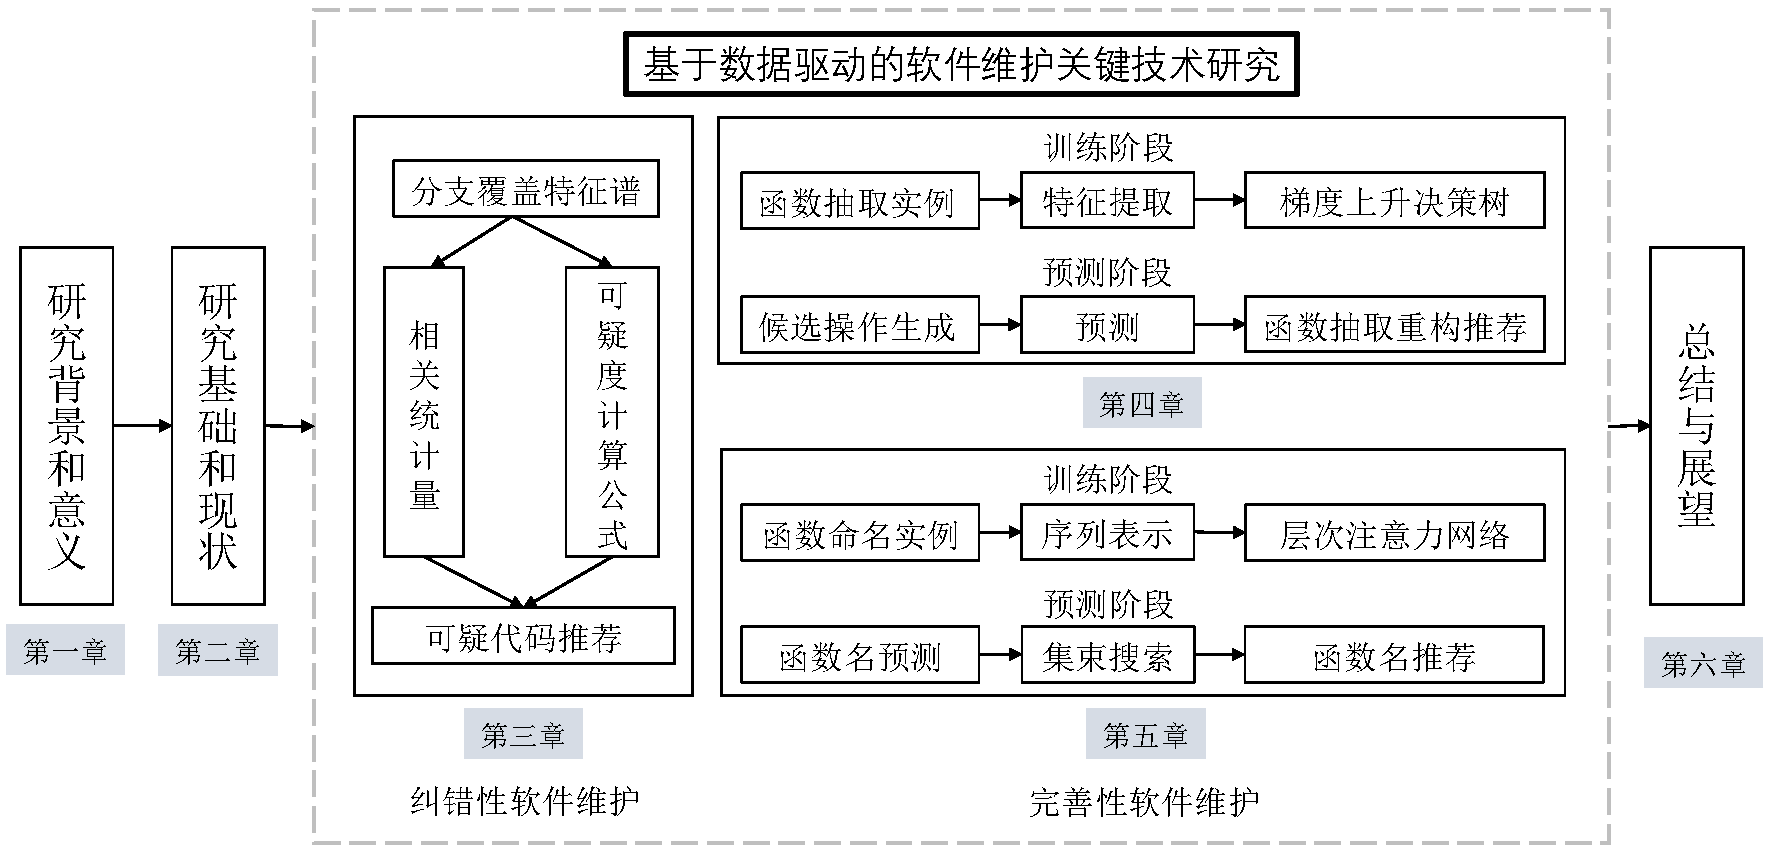
\includegraphics[width=1.0\linewidth]{org.pdf}
  \caption{论文组织结构}
  \label{fig:org}
\end{figure}

如图~\ref{fig:org}所示,本文共分为六章。首先,第一章介绍了本文研究的背景和意义,以及本文的主要研究内容和创新点。后续章节的内容如下:  

第二章介绍本文的研宄基础与现状。本文针对的两种主要的软件维护类型,即纠错性维护和完善性维
护,进行研究。本文首先介绍了缺陷定位相关研究现状;然后介绍了软件重构的相关基础,包括软件质量和代码坏味的关系、软件重构操概述和软件重构推荐方法的研究现状。

第三章提出了基于Relief特征选择的缺陷定位方法。首先介绍了基于分支覆盖特征谱的缺陷定位方法的一般流程,然后介绍了相关统计量的概念和方法。接着使用相关统计量来推测代码覆盖信息对测试用例执行结果的重要性,将其作为可疑度的辅助计算方法,与Ochiai可疑度相结合。最后将代码按照可疑度排序,由高至低推荐给用户。

第四章提出了基于梯度上升决策树的函数抽取重构机会推荐方法。首先介绍了使用梯度上升决策树进行二分类的原理,然后介绍了本文的梯度上升决策树分类和逻辑斯特回归融合模型,接着介绍函数抽取重构实例数据收集方法以及特征提取算法。在预测阶段,介绍了基于代码块的候选重构操作生成,并基于预测结果排序。最后介绍了本文的实验部分,包括实验数据集和评价指标,以及在不同模型和数据集上的实验结果。

第五章提出了基于层次注意力的函数名推荐方法。首先介绍了层次结构的代码片段表示方法,然后介绍了层次注意力模型和集束搜索(Beam Search)在模型中的应用。最后描述了本文的实验部分,包括实验数据集和评价标准,以及与其它经典的函数命名方法的对比实验结果。

第六章对本文进行总结,并展望接下来的研究方向。

\chapter{研究基础和现状}
本章首先介绍了纠错性软件维护的相关工作,包括缺陷定位和缺陷预测等;然后介绍了完善性软件维护的研究基
础,包括软件质量和代码坏味的关系、软件重构操概述和软件重构推荐方法等。
\section{纠错性软件维护}
纠错性软件维护是保证软件系统正确性的重要手段,本节主要介绍缺陷定位的相关研究工作,并简单介绍其它纠错
性软件维护,如缺陷预测。
\subsection{缺陷定位}
软件缺陷是导致软件系统行为与预期不一致的主要原因。为了帮助软件维护人员迅速消除缺陷,首要任务就是找到
软件缺陷在源代码中的位置,即缺陷定位。当软件失效时,缺陷定位是保障软件系统正确性的重要手段。缺陷定位
方法主要有覆盖分析、程序切片、依赖分析、程序不变量等。

(1)覆盖分析法

覆盖分析指的是根据程序执行过程中的覆盖统计信息,按照特定的可疑度计
算公式计算代码可疑度,并按照可疑度高低排序推荐的过程。由于覆盖分析的计算成本低,准确性较高,因此得到
了广泛的关注。其核心思想是,被失效用例执行越多、成功用例执行越少的代码可疑度越高
~\cite{jones2005empirical}。

基于覆盖分析的缺陷定位,其一般过程是首先执行测试用例,收集测试用例对程序元素(如语句、谓词或分支等)
的覆盖信息并统计执行结果(失效或成功),然后使用特定的可疑度计算公式计算可疑度,并将程序元素按照可疑
度由高至低排序,推荐给软件维护人员进行缺陷定位。基于覆盖分析的缺陷定位,其流程大多相似,主要区别在于
可疑度计算公式。表~\ref{fig:susp}中展示了较为经典的六种可疑度计算公式,为了便于理解,所有公式都沿用
Tarantula中的变量定义。Ochiai公式最先在生物学中作为基因相似度的度量公式被提出,Abreu等人
~\cite{abreu2007accuracy}将其运用到可疑度计算中,并得到不错的表现。同时,受聚类分析的启发,他们提出
使用相似度系数Jaccard来度量程序代码的可疑度~\cite{abreu2007accuracy}。Wong等人
~\cite{wong2008crosstab}提出基于交叉表的方法计算代码可疑度,认为覆盖某个程序元素的测试用例,其被失效
执行次数越多,成功执行次数越少,则该程序元素越可能包含缺陷。该方法通过计算相同程序元素被失效执行和成
功执行的相差次数来计算可疑度。Kulczynski公式最早出现在生物学中~\cite{willett2003similarity},Wong等
人~\cite{wong2014dstar}将其扩充后用来计算代码可疑度,其借助失效用例的相似性来进行缺陷定位,在实验数
据集上得到了较高的准确度。Naish等人~\cite{naish2011model}对比了36种基于覆盖分析的缺陷定位方法,根据
实验结果将这些覆盖分析法的可疑度计算公式分为组,每组的计算公式互相等价,并得到Optimal排序方法较其它
方法表现更好的结论。

\begin{center}
\tablecaption{经典可疑度计算公式}\label{fig:susp}
\begin{tabular}{|c|c|}
\hline
覆盖分析法 & 可疑度计算公式 \\ \hline
Tarantula & $\frac{\frac{a_{11}}{a_{11}+a_{01}}}{\frac{a_{11}}{a_{11}+a_{01}}+\frac{a_{10}}{a_{10}+a_{00}}}$\\ 
Jaccard & $susp = \frac{a_{11}}{a_{11}+a_{01}+a_{10}}$\\ 
Ochiai & $susp = \frac{a_{11}}{\sqrt{(a_{11}+a_{01})\times(a_{11}+a_{10})}}$\\
Ochiai2 & $susp = \frac{a_{11}a_{10}}{\sqrt{(a_{11}+a_{10})\times (a_{00}+a_{10})\times (a_{11}+a_{01})\times (a_{01}+a_{00})}}$\\ 
Wong & $susp = a_{11}-a_{10}$\\
DStar & $susp = \frac{a_{11}^{star}}{a_{10}+a_{01}}$\\ 
Naish2 & $susp = a_{11}-\frac{a_{10}}{a_{10}+a_{00}+1}$ \\
Optimal & $susp = \begin{cases}
  -1, & \text{ if } a_{01}>0 \\ 
  a_{00}, & \text{ elsewise }  
  \end{cases}$\\ \hline
\end{tabular}
\end{center}





(2)程序切片法


(3)依赖分析法

(4)其它方法

在缺陷定位方面,张云乾等人~\cite{malcov2013}认为缺陷定位技术的准确性和错误类型有关,因此提出使用马尔
科夫模型预测错误类型,然后选用有针对性的缺陷定位技术进行缺陷定位。何加浪和张宏~\cite{nnfault2013}通
过建立神经网络学习错误和输入之间的关系,通过计算程序中每个位置对错误的支持度来进行多缺陷定位。

\subsection{缺陷预测}

在缺陷预测方面,Menzies等人~\cite{menzies2007data}使用朴素贝叶斯模型进行缺陷预测,并提出在预处理阶
段,使用对数操作可以提升缺陷预测能力。Drown等人~\cite{drown2009evolutionary}提出了基于遗传算法的缺陷
预测模型,利用遗传算法中的指标优化采样过程。Khoshgoftaar等人~\cite{khoshgoftaar2010attribute}提出结
合特征选择和采样的模型来进行缺陷预测。
\section{完善性软件维护}

\subsection{代码坏味}
代码坏味是软件系统中出现``坏代码''的信号,通常被研究者认为软件系统需要进行重构的信号。Fowler等人提出
了22种软件结构作为代码坏味的表现,并认为这些代码坏味可以帮助软件维护人员决定软件是否需要被重构
~\cite{fowler1999refactoring}。同时,Fowler等人提出了72代码重构操作,在保持程序外在行为的一致性的同
时,改进程序内部的设计结构~\cite{fowler1999refactoring}。在表~\ref{fig:badsmell}中我们列举了其中十种
经典的代码坏味,以及可能解决这些代码坏味的软件重构操作。

\begin{center}
\tablecaption{十种经典代码坏味}\label{fig:badsmell}
\begin{tabular}{|l|l|l|l|}
\hline
序号 & 代码坏味 & 软件重构操作 & 重构目标\\ \hline
1 & 代码重复 & 函数提炼、函数上移、类提炼 & 提取公共代码\\ \hline
2 & 函数过长 & 函数提炼 & 拆分函数\\ \hline
3 & 类过大 & 类提炼 & 拆分类\\ \hline
4 & 参数过多 & 引入参数对象、函数替代参数 & 减少参数\\ \hline
5 & 发散式变化& 类提炼 & 将全部变化提取到新类\\ \hline
6 & 霰弹式改动& 函数移动、类内联 & 将全部修改合并为同类\\ \hline
7 & 依恋情节& 函数提炼、函数移动 & 移动依恋代码\\ \hline
8 & 数据泥团& 类提炼、引入参数对象 & 简化数据\\ \hline
9 & 基本类型偏执& 对象替换数据 & 简化类型 \\ \hline
10 & Switch语句 & 函数提炼、函数移动 & 减少Switch语句\\ \hline
\end{tabular}
\end{center}

值得注意的是,每一种代码坏味可以被一种或多种软件重构操作所解决。如表~\ref{fig:badsmell}中的代码重
复,在很多情况下可以通过函数提炼(Extract Method)提取重复的代码结构作为一个新的函数被调用;当重复代
码出现在两个兄弟子类时,可以分别在这两个子类中进行函数提炼,然后将该函数上移(Pull Up Method)到这两
个子类的父类中;当重复代码出现在两个不相干的类中时,可以将重复代码提取为一个新类(Extract Class),
在原来的两个类中调用这个新类。因此我们可以看出,即使针对同一代码坏味,在不同的情况下软件维护人员需要
选择不同的重构操作,甚至是一系列重构操作的叠加。

代码坏味不完全是相互独立的,有一些代码坏味是相关联的,因此可以被相同的软件重构操作所解决。例如代码重
复可能会导致函数过长或者类过大,此时如果使用函数提炼或类提炼,既解决了代码重复的问题,同时也解决了函
数过长或者类过大的问题。同样,依恋情节通常发生在某个函数对某个类的兴趣远高于其所在的类,此时会导致该
函数频繁的访问该类,可能导致函数过长、类过大、参数过多以及发散式变化(容易受到该类的影响)等代码坏
味。通过将部分依恋代码提炼成新的函数,并移动到其频繁访问的类(Move Method),可以让大部分问题得到改
善。

有一些代码坏味是互斥的,因此它们所对应的软件重构操作也是互为逆向操作。如表~\ref{fig:badsmell}中的类
过大和霰弹式改动是两个互斥的代码坏味。当我们用类提炼将大类拆分成多个小类时,虽然每个类的规模变小,但
容易引发霰弹式改动的问题,即原来在同一个大类中的多个小类由于彼此依赖,导致当改动其中一个小问题时,引
发一系列发散的改动,造成软件维护的不便;反之,当我们用类内联(Inline Class)将某个修改所涉及到的修改
都集合到同一个大类中时,虽然解决了霰弹式改动的代码坏味,但此时容易引起类过大的问题。这样逆向的软件重
构操作还有函数提炼和函数内联(Inline Method)、函数上移和函数下移(Pull Down Method)等。因此,如何
针对软件系统选取合适的软件重构操作是软件维护人员需要解决的问题。

虽然代码坏味是软件重构的重要信号,但是软件重构的动机却不完全是为了解决代码坏味。Silva等人
~\cite{silva2016we}调查研究了软件开发人员进行软件重构的动机。调查发现,软件重构主要发生在需求发生改变
的时候,如增加新特性或是修复软件错误时,因此软件重构的动机通常与提高软件的易读性、可重用性、易测性等
相关,而不仅仅是针对特定代码坏味的修复。以最常用的软件重构操作--函数提炼为例,调查显示,软件维护人员
进行函数提炼重构的原因较为复杂,包括代码重用、函数分解、加速扩展、重命名内部函数等11种主要原因。其
中,只有函数分解与代码坏味有关,其通常被认为是决代码坏味``函数过长''的方法。由于人工识别软件重构机会
并选择软件重构操作的成本较高,且软件重构的动机具有复杂性和多样性,研究者们提出了很多软件重构推荐技术
来解决该问题,关于软件重构推荐的研究引起了广泛关注。

\subsection{软件重构原理概述}

软件重构提高软件质量,降低软件维护成本的重要手段之一。重构这个术语最早由William
Opdyke~\cite{opdyke1992refactoring}在其博士论文中提出的。软件重构技术旨在在不改变软件整体功能的前提
下,改进软件的设计结构,使得新的设计结构提高代码的可维护性,从而提高软件的质量
~\cite{fowler1999refactoring}。因此,软件重构通常只改变软件的外观,比如在传统的结构化设计上以改进其
结构。软件重构不涉及修改软件的语义和功能,而是通过更好的观察软件系统,从而提出对软件系统设计各方面的
改进~\cite{chikofsky1990reverse}。

\begin{figure}
  \centering
  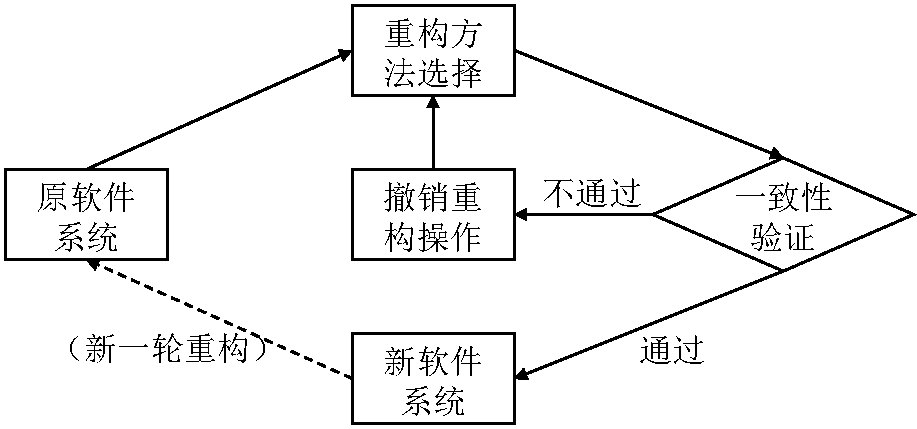
\includegraphics[height=45mm, width=90mm]{refactory.pdf}  
  \caption{\label{fig:refactory}软件重构一般过程}
\end{figure}

软件重构的一般是通过迭代转换的方式对软件系统进行转换。图~\ref{fig:refactory}描述了这样的转换过程。针
对原软件系统,每一轮迭代是对软件的一次小规模转换,针对特定代码选择某种重构方法,在实施软件重构操作后
测试其正确性,即测试软件的语义和功能是否与原来的保持一致。若测试通过,则本轮重构完成,软件维护人员可
在新的软件系统上进行新一轮重构。在任何时间一旦测试不通过,则最后一次程序转换撤销,需要重新选择重构方
法,换一种方式进行重构。通过很多轮这样的小规模程序转换,软件重构的过程和细节可以完全被软件维护人员所
掌控,并达到其所预想的效果。这样的迭代过程要求测试过程十分迅速,否则软件维护人员将不得不花费大量的时
间等待测试完成。因此,很多极限编程和其它敏捷软件开发的使用者将这种迭代过程作为软件开发周期的一个重要
组成部分。除此以外,为了减少一致性验证所带来的测试时间成本,部分学者提出使用先置性条件过滤,使得满足
条件的软件重构能保持语义和功能的一致性,从而减少不必要的测试成本。

软件重构是影响软件完善性维护的重要方面。在软件生命周期中,新的需求被不断添加,使得代码的复杂度越来越
高,代码结构逐渐偏离原来的设计,从而导致了扩展软件的难度越来越大。软件重构增加了程序设计的灵活性,通
过改进软件设计,使得软件具备高内聚、低耦合和复杂度低等特点,将复杂代码变简单,从而提高代码的可扩展
性,降低软件的维护成本。完善性软件维护的时机通常与软件系统质量有关。软件质量下降时,软件系统发出需要
重构的信号。最常见的情况是当软件维护人员修补错误或添加新功能时,首先要需要做的就是理解代码。当代码可
读性强,容易被理解时,修复软件错误和添加新功能的效率更高。相反,当代码复杂度高、不容易被理解时,代码
的质量下降,可维护性也随之降低,此时通常需要对软件进行重构。完善性软件维护可以加速当前和未来对代码的
理解,从而提高软件维护效率。

\subsection{软件重构检测}
软件重构检测通过检测相同软件系统不同版本之间发生的软件重构操作,帮助软件维护人员熟悉代码改变的意图,
更好地了解软件的演化过程。Robbes等人~\cite{robbes2008spyware}开发了一个工具集Spyware来监视集成开发环
境。该工具将软件开发人员对代码的修改表示为基于语义的修改序列,并将这些重要的修改存储起来,开发者可以
通过观察和重放这些修改来观测到软件重构的发生。

大多数研究者主要通过比较两个软件版本中代码的相似度来检测软件重构。Demeyer等人
~\cite{demeyer2000finding}首次提出通过比较相同软件系统的不同版本来检测软件重构的方法,该方法通过比较
软件度量,如代码行数(LOC)和函数调用个数等,检测是否存在软件重构。Malpohl等人
~\cite{malpohl2003renaming}通过使用diff命令来比较两个函数的相似度,从而推测出函数重命名的重构操作。
Antoniol等人~\cite{antoniol2004automatic}提出了基于向量空间的信息检索方法检测代码重构。Xing等人
~\cite{xing2005umldiff}基于命名和结构相似度,自上之下比较了包、类、借口等程序元素。同样基于相似度原
理,部分研究者将克隆检测器应用于软件重构检测中,将不同版本的函数相对应,从而检测出函数提炼和函数移动
等软件重构操作~\cite{van2003reconstruction,kim2005functions}。Weißgerber等人
~\cite{weissgerber2006identifying}提出将软件仓库通过预处理存储进关系型数据库中,然后将每次提交的代码
修改作为事务创建,从中分析出增加、修改或删除的类、字段和函数,从而得到可能的软件重构操作,最后使用克
隆检测将这些操作排序。

由于软件重构的本质是保持软件的语义不变,改变其内部结构,因此有研究者提出使用基于语义分析的方法检测软
件重构。Dig等人~\cite{dig2006automated}开发了基于Eclipse的插件,其首先通过语义分析函数调用、类型使
用、实例化等关系,然后使用一种迭代的方法自顶而下的检测重构。Fluri等人~\cite{fluri2007change}比较了两
个版本的抽象语法树,计算了基于抽象语法树的修改操作,并将其映射到抽象语法树级别的代码修改上。这种方法
的优点在于识别了语法树级别的原子改变,但是由于其停留在原子改变,而未将多处改变抽象化分析,导致其很难
检测出更抽象级别的软件重构。

由于基于相似度比较的软件重构检测方法,其侧重点在于不同版本的软件系统的比较,导致其所能检测出的软件重
构的类型有限,大多为函数移动、函数重命名等简单的重构类型;而复杂重构类型往往涉及多处修改,因此很难被
基于相似度比较的方法检测到。Taneja等人~\cite{taneja2007automated}开发了一种工具RefacLib,通过句法分
析来检测代码库的不同版本之间可能存在的软件重构操作。Kim等人~\cite{kim2007automatic}提出了一种基于规
则的识别代码修改的方法,发现并总结了代码改变的逻辑规则,通过自动匹配不同软件系统的函数并根据该逻辑规
则检测软件重构。Xing等人~\cite{xing2006refactoring}将32种特定类型的软件重构表示成查询语句,提出了基
于代码改变的查询方法,将不同软件版本在软件设计的改变提取到数据库中,查询满足软件重构规则的重构操作实
例。Prete等人~\cite{prete2010template}提出了基于逻辑的方法来检测软件重构,根据模板逻辑规则将每个重构
类型表示出来,并使用逻辑编程引擎来推测重构实例。他们开发了工具Ref-Finder,从代码结构上分析了63种软件
重构类型所对应的重构前后的改变。


\subsection{软件重构机会推荐}

研究者们提出了很多面向软件重构的技术和工具,主要可以分为两类:手动和自动化的方法。第一类方法主要第二类方法通过自动推荐可以被软
件维护人员直接采用的重构序列来提高软件质量\cite{harman2007pareto, kessentini2011design,
ouni2013maintainability, Silva2014}。这种序列可以是一个完整的重构方案,即软件维护人员必须接受完整的
解决方案;也可以是针对特定重构类型的推荐序列,维护人员可以通过逐步交互的方法来完全控制他们所要应用的
重构,通过有针对性的修复来提高软件质量。

软件重构的一般过程是选定待重构代码,然后选择软件重构操作,在进行重构后对软件的一致性进行检测,确保该
软件重构操作没有改变软件原有的语义和功能。由于软件重构原因和过程的复杂性,导致软件维护人员需要根据自
己对软件系统的理解,不断做出决策,耗费大量的时间和精力成本。尤其是当重构操作涉及到不止一个文件和代码
包时~\cite{liu2013monitor},因此,自动软件重构技术越来越得到研究者们的关注。本节首先介绍软件重构操作
的自动检测技术,然后介绍软件重构推荐的相关技术,包括软件重构机会的识别和推荐,以及软件重构顺序推荐,
最后介绍软件重构的一致性相关研究。


虽然半自动的软件重构过程可以省去不必要的人工操作和验证,但其仍然依赖于程序员对软件系统的理解来做出一
系列适合当前软件系统的决策。为了提高软件重构效率,已经有很多工作致力于软件重构机会的识别和推荐。关于
软件重构机会推荐的工作通常包括两个方面,分别是软件重构机会的识别和软件重构操作推荐。这两个方面分别对
应着软件重构的两个关键步骤:(1)识别选定代码是否存在软件重构机会(2)为选定代码推荐合适的软件重构操
作。通常情况下,只有识别了软件重构机会,才有可能对软件进行重构。而人工识别软件重构机会往往要求软件维
护人员对软件系统的设计和实现有全局的了解,因此对软件维护人员的经验和能力要求较高,尤其是在不用程序分
析工具的情况下,了解软件系统的设计并识别软件重构机会是一个复杂而耗时的过程。值得注意的是,部分研究将
这两个步骤融合在一起,在识别软件重构机会的同时推荐重构操作。例如,当我们对代码进行克隆检测
~\cite{kamiya2002ccfinder}的同时,如果我们检测到了克隆代码,往往使用函数提炼或类提炼等重构将公共代码
提取出来,以便复用。根据主要方法的不同,我们可以将关于软件重构机会推荐的研究分为六类
~\cite{al2015identifying}。

 
\iffalse
\subsubsection{基于软件质量度量的重构机会推荐}
\subsubsection{基于前置条件的重构机会推荐}
\subsubsection{基于聚类的重构机会推荐}
\subsubsection{基于图的重构机会推荐}
\subsubsection{基于代码切片的重构机会推荐}
\subsubsection{基于动态分析的重构机会推荐}
\subsection{软件重构顺序推荐}
\fi
